\documentclass[tikz,border=10pt]{standalone}
\usepackage{helvet}
\renewcommand{\familydefault}{\sfdefault}
\usepackage{tikz}
\usetikzlibrary{positioning, arrows.meta, shapes.geometric, calc, fit, backgrounds, decorations.pathreplacing}

\definecolor{emeraldpine}{HTML}{1A4D3E}
\definecolor{harvardcrimson}{HTML}{A51C30}
\definecolor{ethdarkblue}{HTML}{1F407A}
\definecolor{ethpetrol}{HTML}{007A87}
\definecolor{ethbronze}{HTML}{B87333}
\definecolor{ethpurple}{HTML}{5B4B8A}
\definecolor{ink}{HTML}{1A202C}
\definecolor{softink}{HTML}{4A5568}
\definecolor{paleink}{HTML}{A0AEC0}
\definecolor{cardbg}{HTML}{F8FAFC}
\definecolor{shadecolor}{HTML}{F4F6F9}

\begin{document}
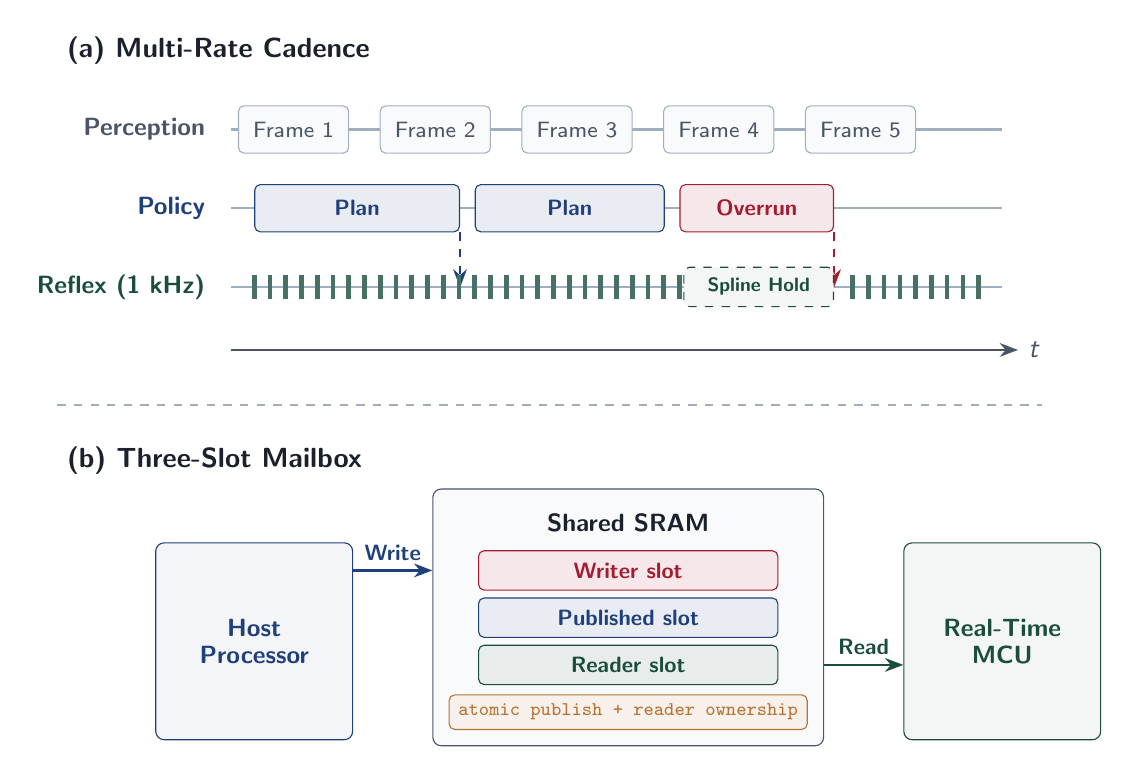
\begin{tikzpicture}[
    font=\sffamily,
    >=Stealth,
    node distance=1.5cm and 2cm,
    framebox/.style={
        rectangle, rounded corners=2pt, draw=paleink, fill=cardbg,
        minimum height=0.6cm, minimum width=1.5cm, align=center,
        font=\fontsize{8}{9}\selectfont\color{softink}
    },
    planbox/.style={
        rectangle, rounded corners=2pt, draw=ethdarkblue, fill=ethdarkblue!10,
        minimum height=0.6cm, minimum width=2.5cm, align=center,
        font=\fontsize{8}{9}\selectfont\color{ethdarkblue}\bfseries
    },
    overrunbox/.style={
        rectangle, rounded corners=2pt, draw=harvardcrimson, fill=harvardcrimson!10,
        minimum height=0.6cm, minimum width=1.8cm, align=center,
        font=\fontsize{8}{9}\selectfont\color{harvardcrimson}\bfseries
    },
    holdbox/.style={
        rectangle, rounded corners=2pt, draw=emeraldpine, fill=emeraldpine!5,
        minimum height=0.5cm, minimum width=1.8cm, align=center, dashed,
        font=\fontsize{7}{8}\selectfont\color{emeraldpine}\bfseries
    },
    slotbox/.style={
        rectangle, rounded corners=2pt, draw=#1, fill=#1!10,
        minimum height=0.5cm, minimum width=3.8cm, align=center,
        font=\fontsize{8}{9}\selectfont\color{#1}\bfseries
    },
    procbox/.style={
        rectangle, rounded corners=3pt, draw=#1, fill=#1!5,
        minimum height=2.5cm, minimum width=2.5cm, align=center,
        font=\fontsize{9}{10}\selectfont\color{#1}\bfseries
    },
    srambox/.style={
        rectangle, rounded corners=3pt, draw=softink, fill=cardbg,
        minimum height=2.5cm, minimum width=4.5cm, align=center
    }
]

% ==========================================
% PANEL (a): Multi-Rate Cadence
% ==========================================
\node[font=\fontsize{10}{12}\selectfont\bfseries\color{ink}, anchor=west] at (0, 0) {(a) Multi-Rate Cadence};

% Row Labels
\node[anchor=east, font=\fontsize{9}{10}\selectfont\bfseries\color{softink}] at (2, -1) {Perception};
\node[anchor=east, font=\fontsize{9}{10}\selectfont\bfseries\color{ethdarkblue}] at (2, -2) {Policy};
\node[anchor=east, font=\fontsize{9}{10}\selectfont\bfseries\color{emeraldpine}] at (2, -3) {Reflex (1 kHz)};

% Timelines
\draw[paleink, thick] (2.2, -1) -- (12, -1);
\draw[paleink, thick] (2.2, -2) -- (12, -2);
\draw[paleink, thick] (2.2, -3) -- (12, -3);

% Time Axis
\draw[softink, thick, ->] (2.2, -3.8) -- (12.2, -3.8) node[right, font=\itshape\color{softink}] {t};

% Perception Frames
\node[framebox, minimum width=1.4cm] (f1) at (3.0, -1) {Frame 1};
\node[framebox, minimum width=1.4cm] (f2) at (4.8, -1) {Frame 2};
\node[framebox, minimum width=1.4cm] (f3) at (6.6, -1) {Frame 3};
\node[framebox, minimum width=1.4cm] (f4) at (8.4, -1) {Frame 4};
\node[framebox, minimum width=1.4cm] (f5) at (10.2, -1) {Frame 5};

% Policy Plans
\node[planbox, minimum width=2.6cm, anchor=west] (p1) at (2.5, -2) {Plan};
\node[planbox, minimum width=2.4cm, anchor=west] (p2) at (5.3, -2) {Plan};
\node[overrunbox, minimum width=1.95cm, anchor=west] (p3) at (7.9, -2) {Overrun};

% Handoff Arrows
\draw[->, ethdarkblue, thick, dashed] (p1.south east) -- ++(0, -0.7);
\draw[->, harvardcrimson, thick, dashed] (p3.south east) -- ++(0, -0.7);

% Reflex Ticks (using a loop)
\foreach \x in {2.5, 2.7, 2.9, 3.1, 3.3, 3.5, 3.7, 3.9, 4.1, 4.3, 4.5, 4.7, 4.9, 5.1, 5.3, 5.5, 5.7, 5.9, 6.1, 6.3, 6.5, 6.7, 6.9, 7.1, 7.3, 7.5, 7.7, 7.9} {
    \fill[emeraldpine!80] (\x-0.03, -3.15) rectangle (\x+0.03, -2.85);
}

% Overrun Hold Capsule
\node[holdbox, minimum width=1.9cm, anchor=west] (hold) at (7.95, -3) {Spline Hold};

% Resumed Reflex Ticks
\foreach \x in {10.1, 10.3, 10.5, 10.7, 10.9, 11.1, 11.3, 11.5, 11.7} {
    \fill[emeraldpine!80] (\x-0.03, -3.15) rectangle (\x+0.03, -2.85);
}

% Divider
\draw[paleink, thick, dashed] (0, -4.5) -- (12.5, -4.5);

% ==========================================
% PANEL (b): Three-Slot Mailbox
% ==========================================
\node[font=\fontsize{10}{12}\selectfont\bfseries\color{ink}, anchor=west] at (0, -5.2) {(b) Three-Slot Mailbox};

% Host Processor
\node[procbox=ethdarkblue] (host) at (2.5, -7.5) {Host\\Processor};

% Shared SRAM elements
\node[slotbox=harvardcrimson] (slot1) at (7.25, -6.6) {Writer slot};
\node[slotbox=ethdarkblue] (slot2) at (7.25, -7.2) {Published slot};
\node[slotbox=emeraldpine] (slot3) at (7.25, -7.8) {Reader slot};

\node[rectangle, rounded corners=2pt, draw=ethbronze, fill=ethbronze!10, minimum height=0.4cm, minimum width=3.8cm, align=center, font=\fontsize{7}{8}\selectfont\ttfamily\color{ethbronze}\bfseries] (rule) at (7.25, -8.4) {atomic publish + reader ownership};

\node[font=\fontsize{9}{10}\selectfont\bfseries\color{ink}] (sramtitle) at (7.25, -6.0) {Shared SRAM};

% Draw Shared SRAM box in background
\begin{scope}[on background layer]
    \node[rectangle, rounded corners=3pt, draw=softink, fill=cardbg, fit=(sramtitle) (slot1) (slot2) (slot3) (rule), inner sep=0.2cm] (sram) {};
\end{scope}

% Real-Time MCU
\node[procbox=emeraldpine] (mcu) at (12, -7.5) {Real-Time\\MCU};

% Arrows
\draw[->, ethdarkblue, thick] (host.east |- slot1) -- (sram.west |- slot1) node[midway, above, font=\fontsize{8}{9}\selectfont\bfseries\color{ethdarkblue}] {Write};
\draw[->, emeraldpine, thick] (sram.east |- slot3) -- (mcu.west |- slot3) node[midway, above, font=\fontsize{8}{9}\selectfont\bfseries\color{emeraldpine}] {Read};

\end{tikzpicture}
\end{document}
